%%% PREAMBLE - Do not touch %%%%%%%%%%%%%%%%%%%%%%%%%%%%%%%%%%%%%%%%%%%%%%%%%%%%%%
\documentclass[10pt,twocolumn,letterpaper]{article}
\usepackage[utf8]{inputenc}
\usepackage[english]{babel}
\usepackage{model}
\usepackage{times}
\usepackage{epsfig}
\usepackage{graphicx}
\usepackage{amsmath}
\usepackage{textcomp}
\usepackage{amssymb}
\usepackage{color}
\usepackage[pagebackref=true,breaklinks=true,letterpaper=true,colorlinks,bookmarks=false]{hyperref}

%% inset source code
\usepackage{listings}

\lstset{basicstyle=\footnotesize\ttfamily,  language=C}
\renewcommand{\lstlistingname}{Code}% Listing -> Algorithm

\let\url\nolinkurl% Make \url be equivalent to \nolinkurl
\newcommand*{\Package}[1]{\texttt{#1}}%

\cvprfinalcopy % *** Uncomment this line for the final submission
\def\httilde{\mbox{\tt\raisebox{-.5ex}{\symbol{126}}}}
\ifcvprfinal\pagestyle{empty}\fi

\newcommand{\TODO}[1]{TODO: #1}
\newcommand{\CITEONE}[2]{\mbox{#1 \cite{#2}}}
\newcommand{\CITETWO}[3]{\mbox{#1 and #2 \cite{#3}}}
\newcommand{\CITEN}[2]{\mbox{#1 et al. \cite{#2}}}

%%% Report beginning %%%%%%%%%%%%%%%%%%%%%%%%%%%%%%%%%%%%%%%%%%%%%%%%%%%%%%%%%%%%%%
\begin{document}

%%% Title and authors %%%%%%%%%%%%%%%%%%%%%%%%%%%%%%%%%%%%%%%%%%%%%%%%%%%%%%%%%%%%
\title{Relatório da atividade 2.1}
\author{Isadora Sophia Garcia Rodopoulos \thanks{RA 158018, Instituto de Computação, Universidade de Campinas, Unicamp. \textbf{Contact}: \tt\small{isadorasophiagr@gmail.com}} \\
Matheus Mortatti Diamantinos \thanks{RA 156740, Instituto de Computação, Universidade de Campinas, Unicamp. \textbf{Contact}: \tt\small{matdiamantino@gmail.com}}\\
Luiz Fernando Bittencourt\thanks{MC833, Instituto de Computação, Universidade de Campinas, Unicamp. \textbf{Contact}: \tt\small{bit@ic.unicamp.br }}\\
}

%%% Abstrato %%%%%%%%%%%%%%%%%%%%%%%%%%%%%%%%%%%%%%%%%%%%%%%%%%%%%%%%%%%%%%%%%%%%%
\maketitle
\begin{abstract}
O objetivo do trabalho se baseou em modificar a implementação da aplicação cliente-servidor
anterior, substituindo \texttt{fork()} por \texttt{select()}.
\end{abstract}

%%% image for demo! %%%%%%%%%% 
\begin{figure*}
\begin{center}
    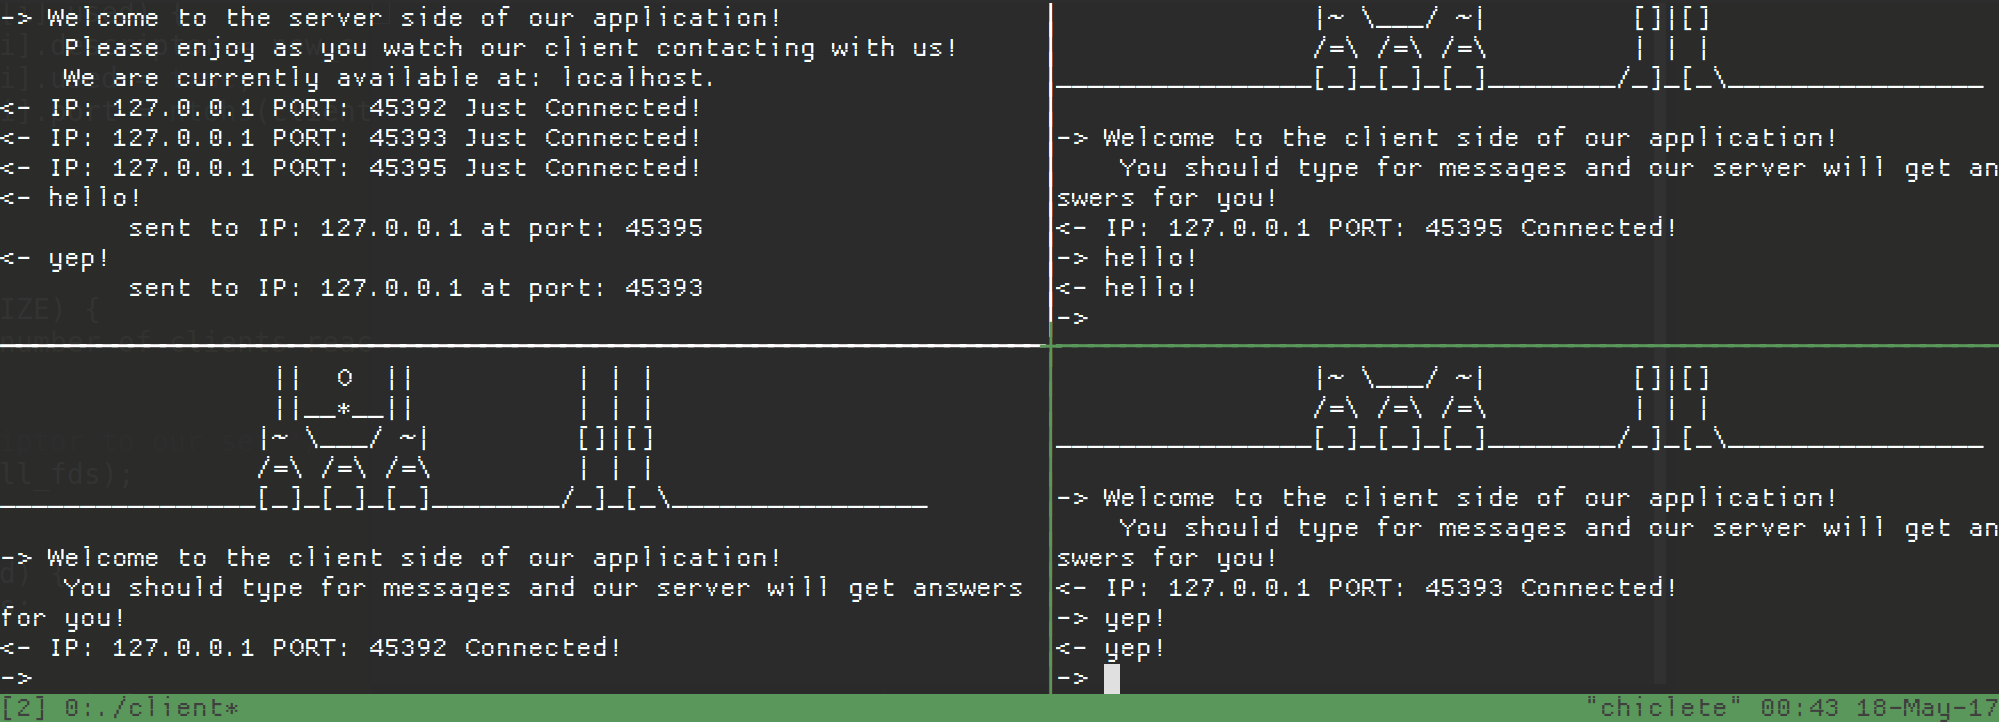
\includegraphics[width=1\textwidth]{img/sample.png}
    \caption{Exemplo de funcionamento do projeto}   
\end{center} 
\end{figure*}
%%%%%%%%%%%%%%%%%%%%%%%%%%%%%%%%%% page 2

%%% Introdução %%%%%%%%%%%%%%%%%%%%%%%%%%%%%%%%%%%%%%%%%%%%%%%%%%%%%%%%%%%%%%%%%%%
Neste projeto, foi implementado uma estrutura de comunicação entre cliente e servidor baseado em uma conexão TCP utilizando sockets na linguagem C. Nela, vários clientes podem se conectar a um mesmo IP, cada um por uma porta diferente. Foi utilizada a estrutura de \texttt{select()} para permitir que vários clientes se conectem simultaneamente.

Além disso, um \textit{ack} é enviado para cada um dos clientes, em formato de \textit{echo}, para certificar que a mensagem chegou com sucesso.

%%% Seções %%%%%%%#####%%%%%%%%%%%%%%%%%%%%%%%%%%%%%%%%%%%%%%%%%%%%%%%%%%%%%%%%%%%
\section{client.c}
O código para o cliente não sofreu nenhuma modificação funcional em relação aos projetos anteriores,
uma vez que o seu comportamento continua o mesmo, basta conectar-se ao IP do servidor e 
a uma porta disponível. Então, imprime a porta e o ip do servidor conectado.

O fluxo de execução de \texttt{client.c} pode ser resumido, portanto, em:

\begin{enumerate}
    \item Criar o socket de conexão;
    \item Estabelecer conexão com o servidor e imprimir porta e ip para o usuário;
    \item Receber mensagem do usuário, mandar ao servidor e esperar resposta;
    \item Se algum erro ocorrer ou o cliente fechar a aplicação, fechar a conexão.
\end{enumerate}


\begin{lstlisting}[caption={Recuperação da porta e IP do servidor conectado}, label=Algorithm]
    /* Get socket IP and Port and show to client */
    struct sockaddr_in server;
    socklen_t server_size = sizeof(server);

    int res = getsockname(s, 
        (struct sockaddr *)&server, &server_size);

    char ip[INET_ADDRSTRLEN+1];
    inet_ntop(AF_INET, &(client.sin_addr), 
        ip, INET_ADDRSTRLEN);
    ip[INET_ADDRSTRLEN] = '\0';

    /* print text on screen */
    fprintf(stdout, "<- IP: s PORT: d Connected!\n", 
        ip, ntohs(client.sin_port));
\end{lstlisting}

\section{server.c}
Semelhante ao comportamento do programa do cliente, o servidor foi divido em:

\begin{enumerate}
    \item Criar o socket ativo e associá-lo a um descritor;
    \item Enquanto está ativo:
    \begin{enumerate}
        \item Criar um processo filho.
        \item Checar novas conexões de clientes.
        \item Conectar com o cliente e imprimir o IP e a porta da conexão.
        \item Checar mensagens dos clientes ativos. Caso receba uma mensagem, imprimi-la e retornar o \textit{echo}, especificando o IP e o port do cliente.
        \item Caso um cliente se desconecte, fechar a conexão e desalocar o espaço do cliente.
    \end{enumerate}
\end{enumerate}

    Foi estabelecida uma interface bem simples, que permite que o usuário veja as mensagens que serão ecoadas na tela - as quais correspondem às mensagens que o cliente envia através da conexão com o servidor.

\subsection{Criar o socket ativo e associá-lo a um descritor;}

Do mesmo modo que foi feito no cliente, foi criado um socket com a família da qual o endereço pertence (no nosso caso, IPv4), o seu respectivo port de \textit{listening} e o IP, \textit{localhost}. A associação do socket ao descritor se dá a partir da função \textit{bind()}.

Caso ocorra algum erro ou o socket não consiga aceitar nenhuma conexão, um erro é emitido e o programa é finalizado.

\subsection{Enquanto está ativo...}
\subsection{Criar um processo filho}
Utilizou-se a função \texttt{fork()} para criar um processo filho que verifica se uma nova conexão é estabelecida.
\subsubsection{Checar novas conexões de clientes;}

\begin{lstlisting}[caption={Estabelecimento de conexão a um novo cliente}, label=Algorithm]
/* Connect to client and 
show IP and Port of the connection */
int32_t conn = accept(s, 
    (struct sockaddr*) NULL, NULL);
valid(conn, "Failed to establish a connection 
from socket.\n");
\end{lstlisting}

    Do mesmo modo que nos projetos anteriores, checamos se o socket por uma nova conexão e conectamos.

\subsection{Conectar com o cliente e imprimir o IP e a porta da conexão.}

\begin{lstlisting}[caption={Recuperação de IP e Porta do cliente}, label=Algorithm]
/* Connect to client and show 
IP and Port of the connection */
struct sockaddr_in client;
socklen_t client_size = sizeof(client);

int res = getpeername(conn, 
(struct sockaddr *)&client, &client_size);

char ip[INET_ADDRSTRLEN+1];
inet_ntop(AF_INET, &(client.sin_addr), 
ip, INET_ADDRSTRLEN);
ip[INET_ADDRSTRLEN] = '\0';

/* print text on screen */
fprintf(stdout, "<- IP: s PORT: d Just Connected!\n", 
ip, ntohs(client.sin_port));
\end{lstlisting}

Utilizando as funções acima, recuperamos o \texttt{peername} da conexão e imprimimos o IP e a Porta da conexão.

\subsubsection{Checar mensagens dos clientes ativos. Caso receba uma mensagem, imprimi-la e retornar o \textit{echo}, especificando o IP e o port do cliente;}

    Como temos vários processos filhos rodando concorrentemente o mesmo código, não houveram modificações nessa parte com relação ao projeto 1. Apenas imprimiu-se o IP de quem mandou
    a mensagem ao servidor no terminal:

\begin{lstlisting}[caption={Impressão da porta de quem manda a mensagem}, label=Algorithm]
/* print message on screen and destination IP */
fprintf(stdout, "<- %s\tSent To: %s\n", buff, ip);
\end{lstlisting}

\subsection{Comportamentos inesperados}

Caso um cliente se desconecte, fechar a conexão e desalocar o espaço do cliente, ou qualquer erro ocorra durante os procedimentos descritos acima, é realizado o tratamento de erro e, caso seja necessário, a aplicação é encerrada imediatamante.

A mesma API utilizada nos projetos anteriores, \texttt{Api.h}, foi utilizada para encapsular as chamadas de erros.

\section{Testes}

Para testar o funcionamento da infraestrutura, foi necessário abrir o processo do servidor e diversos clientes para se conectar ao servidor por diferentes portas. Foram testados tanto os corner quanto edge cases (como nenhum cliente ou muitos clientes se conectando simultaneamente) e foi checado se os erros foram tratados como o apropriado.

Apesar de algumas oscilações entre as conexões dos clientes (por algum motivo, eventualmente alguns programas do cliente não imprimiriam os \textit{ack} do servidor até que a conexão fosse encerrada, por conflitos do próprio OS), o comportamento se manteve dentro o esperado.

%%% References %%%%%%%%%%%%%%%%%%%%%%%%%%%%%%%%%%%%%%%%%%%%%%%%%%%%%%%%%%%%%%%%%
%%
{\small
\bibliographystyle{unsrt}
\bibliography{refs}
}

\end{document}
